% Created by tikzDevice version 0.12.6 on 2025-04-22 13:35:28
% !TEX encoding = UTF-8 Unicode
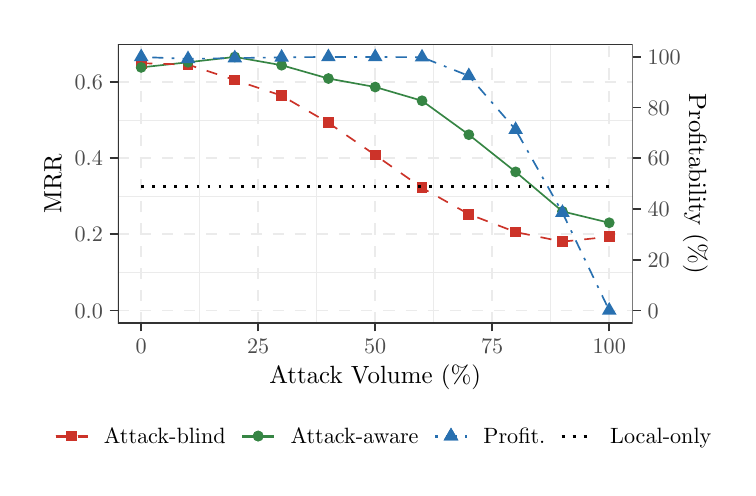
\begin{tikzpicture}[x=1pt,y=1pt]
\definecolor{fillColor}{RGB}{255,255,255}
\path[use as bounding box,fill=fillColor,fill opacity=0.00] (0,0) rectangle (252.94,158.99);
\begin{scope}
\path[clip] (  0.00,  0.00) rectangle (252.94,158.99);
\definecolor{drawColor}{RGB}{255,255,255}
\definecolor{fillColor}{RGB}{255,255,255}

\path[draw=drawColor,line width= 0.6pt,line join=round,line cap=round,fill=fillColor] (  0.00,  0.00) rectangle (252.94,158.99);
\end{scope}
\begin{scope}
\path[clip] ( 32.57, 52.25) rectangle (218.60,152.99);
\definecolor{fillColor}{RGB}{255,255,255}

\path[fill=fillColor] ( 32.57, 52.25) rectangle (218.60,152.99);
\definecolor{drawColor}{gray}{0.92}

\path[draw=drawColor,line width= 0.3pt,line join=round] ( 32.57, 70.58) --
	(218.60, 70.58);

\path[draw=drawColor,line width= 0.3pt,line join=round] ( 32.57, 98.08) --
	(218.60, 98.08);

\path[draw=drawColor,line width= 0.3pt,line join=round] ( 32.57,125.58) --
	(218.60,125.58);

\path[draw=drawColor,line width= 0.3pt,line join=round] ( 62.16, 52.25) --
	( 62.16,152.99);

\path[draw=drawColor,line width= 0.3pt,line join=round] (104.44, 52.25) --
	(104.44,152.99);

\path[draw=drawColor,line width= 0.3pt,line join=round] (146.72, 52.25) --
	(146.72,152.99);

\path[draw=drawColor,line width= 0.3pt,line join=round] (189.00, 52.25) --
	(189.00,152.99);

\path[draw=drawColor,line width= 0.6pt,dash pattern=on 4pt off 4pt ,line join=round] ( 32.57, 56.83) --
	(218.60, 56.83);

\path[draw=drawColor,line width= 0.6pt,dash pattern=on 4pt off 4pt ,line join=round] ( 32.57, 84.33) --
	(218.60, 84.33);

\path[draw=drawColor,line width= 0.6pt,dash pattern=on 4pt off 4pt ,line join=round] ( 32.57,111.83) --
	(218.60,111.83);

\path[draw=drawColor,line width= 0.6pt,dash pattern=on 4pt off 4pt ,line join=round] ( 32.57,139.33) --
	(218.60,139.33);

\path[draw=drawColor,line width= 0.6pt,dash pattern=on 4pt off 4pt ,line join=round] ( 41.02, 52.25) --
	( 41.02,152.99);

\path[draw=drawColor,line width= 0.6pt,dash pattern=on 4pt off 4pt ,line join=round] ( 83.30, 52.25) --
	( 83.30,152.99);

\path[draw=drawColor,line width= 0.6pt,dash pattern=on 4pt off 4pt ,line join=round] (125.58, 52.25) --
	(125.58,152.99);

\path[draw=drawColor,line width= 0.6pt,dash pattern=on 4pt off 4pt ,line join=round] (167.86, 52.25) --
	(167.86,152.99);

\path[draw=drawColor,line width= 0.6pt,dash pattern=on 4pt off 4pt ,line join=round] (210.14, 52.25) --
	(210.14,152.99);
\definecolor{drawColor}{RGB}{54,133,68}

\path[draw=drawColor,line width= 0.6pt,line join=round] ( 41.02,144.63) --
	( 57.94,146.49) --
	( 74.85,148.41) --
	( 91.76,145.42) --
	(108.67,140.61) --
	(125.58,137.54) --
	(142.50,132.58) --
	(159.41,120.32) --
	(176.32,106.88) --
	(193.23, 92.60) --
	(210.14, 88.49);
\definecolor{drawColor}{RGB}{204,51,41}

\path[draw=drawColor,line width= 0.6pt,dash pattern=on 4pt off 4pt ,line join=round] ( 41.02,146.16) --
	( 57.94,145.64) --
	( 74.85,140.08) --
	( 91.76,134.43) --
	(108.67,124.61) --
	(125.58,112.96) --
	(142.50,101.10) --
	(159.41, 91.60) --
	(176.32, 85.14) --
	(193.23, 81.66) --
	(210.14, 83.44);
\definecolor{fillColor}{RGB}{204,51,41}

\path[fill=fillColor] ( 39.06,144.19) --
	( 42.99,144.19) --
	( 42.99,148.12) --
	( 39.06,148.12) --
	cycle;
\definecolor{fillColor}{RGB}{54,133,68}

\path[fill=fillColor] ( 41.02,144.63) circle (  1.96);
\definecolor{fillColor}{RGB}{204,51,41}

\path[fill=fillColor] ( 55.97,143.68) --
	( 59.90,143.68) --
	( 59.90,147.61) --
	( 55.97,147.61) --
	cycle;
\definecolor{fillColor}{RGB}{54,133,68}

\path[fill=fillColor] ( 57.94,146.49) circle (  1.96);
\definecolor{fillColor}{RGB}{204,51,41}

\path[fill=fillColor] ( 72.89,138.12) --
	( 76.81,138.12) --
	( 76.81,142.05) --
	( 72.89,142.05) --
	cycle;
\definecolor{fillColor}{RGB}{54,133,68}

\path[fill=fillColor] ( 74.85,148.41) circle (  1.96);
\definecolor{fillColor}{RGB}{204,51,41}

\path[fill=fillColor] ( 89.80,132.47) --
	( 93.72,132.47) --
	( 93.72,136.40) --
	( 89.80,136.40) --
	cycle;
\definecolor{fillColor}{RGB}{54,133,68}

\path[fill=fillColor] ( 91.76,145.42) circle (  1.96);
\definecolor{fillColor}{RGB}{204,51,41}

\path[fill=fillColor] (106.71,122.64) --
	(110.63,122.64) --
	(110.63,126.57) --
	(106.71,126.57) --
	cycle;
\definecolor{fillColor}{RGB}{54,133,68}

\path[fill=fillColor] (108.67,140.61) circle (  1.96);
\definecolor{fillColor}{RGB}{204,51,41}

\path[fill=fillColor] (123.62,111.00) --
	(127.55,111.00) --
	(127.55,114.93) --
	(123.62,114.93) --
	cycle;
\definecolor{fillColor}{RGB}{54,133,68}

\path[fill=fillColor] (125.58,137.54) circle (  1.96);
\definecolor{fillColor}{RGB}{204,51,41}

\path[fill=fillColor] (140.53, 99.14) --
	(144.46, 99.14) --
	(144.46,103.06) --
	(140.53,103.06) --
	cycle;
\definecolor{fillColor}{RGB}{54,133,68}

\path[fill=fillColor] (142.50,132.58) circle (  1.96);
\definecolor{fillColor}{RGB}{204,51,41}

\path[fill=fillColor] (157.45, 89.64) --
	(161.37, 89.64) --
	(161.37, 93.57) --
	(157.45, 93.57) --
	cycle;
\definecolor{fillColor}{RGB}{54,133,68}

\path[fill=fillColor] (159.41,120.32) circle (  1.96);
\definecolor{fillColor}{RGB}{204,51,41}

\path[fill=fillColor] (174.36, 83.18) --
	(178.28, 83.18) --
	(178.28, 87.10) --
	(174.36, 87.10) --
	cycle;
\definecolor{fillColor}{RGB}{54,133,68}

\path[fill=fillColor] (176.32,106.88) circle (  1.96);
\definecolor{fillColor}{RGB}{204,51,41}

\path[fill=fillColor] (191.27, 79.70) --
	(195.19, 79.70) --
	(195.19, 83.62) --
	(191.27, 83.62) --
	cycle;
\definecolor{fillColor}{RGB}{54,133,68}

\path[fill=fillColor] (193.23, 92.60) circle (  1.96);
\definecolor{fillColor}{RGB}{204,51,41}

\path[fill=fillColor] (208.18, 81.48) --
	(212.11, 81.48) --
	(212.11, 85.40) --
	(208.18, 85.40) --
	cycle;
\definecolor{fillColor}{RGB}{54,133,68}

\path[fill=fillColor] (210.14, 88.49) circle (  1.96);
\definecolor{drawColor}{RGB}{0,0,0}

\path[draw=drawColor,line width= 1.1pt,dash pattern=on 1pt off 3pt ,line join=round] ( 41.02,101.56) --
	(210.14,101.56);
\definecolor{drawColor}{RGB}{40,112,176}

\path[draw=drawColor,line width= 0.6pt,dash pattern=on 1pt off 3pt on 4pt off 3pt ,line join=round] ( 41.02,148.41) --
	( 57.94,147.71) --
	( 74.85,148.00) --
	( 91.76,148.26) --
	(108.67,148.41) --
	(125.58,148.41) --
	(142.50,148.30) --
	(159.41,141.56) --
	(176.32,122.12) --
	(193.23, 92.17) --
	(210.14, 56.83);
\definecolor{fillColor}{RGB}{40,112,176}

\path[fill=fillColor] ( 41.02,151.47) --
	( 43.67,146.89) --
	( 38.38,146.89) --
	cycle;

\path[fill=fillColor] ( 57.94,150.76) --
	( 60.58,146.18) --
	( 55.29,146.18) --
	cycle;

\path[fill=fillColor] ( 74.85,151.05) --
	( 77.49,146.47) --
	( 72.21,146.47) --
	cycle;

\path[fill=fillColor] ( 91.76,151.31) --
	( 94.40,146.73) --
	( 89.12,146.73) --
	cycle;

\path[fill=fillColor] (108.67,151.47) --
	(111.31,146.89) --
	(106.03,146.89) --
	cycle;

\path[fill=fillColor] (125.58,151.47) --
	(128.23,146.89) --
	(122.94,146.89) --
	cycle;

\path[fill=fillColor] (142.50,151.35) --
	(145.14,146.77) --
	(139.85,146.77) --
	cycle;

\path[fill=fillColor] (159.41,144.61) --
	(162.05,140.04) --
	(156.77,140.04) --
	cycle;

\path[fill=fillColor] (176.32,125.17) --
	(178.96,120.59) --
	(173.68,120.59) --
	cycle;

\path[fill=fillColor] (193.23, 95.22) --
	(195.87, 90.64) --
	(190.59, 90.64) --
	cycle;

\path[fill=fillColor] (210.14, 59.88) --
	(212.79, 55.31) --
	(207.50, 55.31) --
	cycle;
\definecolor{drawColor}{gray}{0.20}

\path[draw=drawColor,line width= 0.6pt,line join=round,line cap=round] ( 32.57, 52.25) rectangle (218.60,152.99);
\end{scope}
\begin{scope}
\path[clip] (  0.00,  0.00) rectangle (252.94,158.99);
\definecolor{drawColor}{gray}{0.30}

\node[text=drawColor,anchor=base east,inner sep=0pt, outer sep=0pt, scale=  0.80] at ( 27.17, 54.08) {0.0};

\node[text=drawColor,anchor=base east,inner sep=0pt, outer sep=0pt, scale=  0.80] at ( 27.17, 81.58) {0.2};

\node[text=drawColor,anchor=base east,inner sep=0pt, outer sep=0pt, scale=  0.80] at ( 27.17,109.08) {0.4};

\node[text=drawColor,anchor=base east,inner sep=0pt, outer sep=0pt, scale=  0.80] at ( 27.17,136.58) {0.6};
\end{scope}
\begin{scope}
\path[clip] (  0.00,  0.00) rectangle (252.94,158.99);
\definecolor{drawColor}{gray}{0.20}

\path[draw=drawColor,line width= 0.6pt,line join=round] ( 29.57, 56.83) --
	( 32.57, 56.83);

\path[draw=drawColor,line width= 0.6pt,line join=round] ( 29.57, 84.33) --
	( 32.57, 84.33);

\path[draw=drawColor,line width= 0.6pt,line join=round] ( 29.57,111.83) --
	( 32.57,111.83);

\path[draw=drawColor,line width= 0.6pt,line join=round] ( 29.57,139.33) --
	( 32.57,139.33);
\end{scope}
\begin{scope}
\path[clip] (  0.00,  0.00) rectangle (252.94,158.99);
\definecolor{drawColor}{gray}{0.20}

\path[draw=drawColor,line width= 0.6pt,line join=round] (218.60, 56.83) --
	(221.60, 56.83);

\path[draw=drawColor,line width= 0.6pt,line join=round] (218.60, 75.15) --
	(221.60, 75.15);

\path[draw=drawColor,line width= 0.6pt,line join=round] (218.60, 93.47) --
	(221.60, 93.47);

\path[draw=drawColor,line width= 0.6pt,line join=round] (218.60,111.78) --
	(221.60,111.78);

\path[draw=drawColor,line width= 0.6pt,line join=round] (218.60,130.10) --
	(221.60,130.10);

\path[draw=drawColor,line width= 0.6pt,line join=round] (218.60,148.41) --
	(221.60,148.41);
\end{scope}
\begin{scope}
\path[clip] (  0.00,  0.00) rectangle (252.94,158.99);
\definecolor{drawColor}{gray}{0.30}

\node[text=drawColor,anchor=base west,inner sep=0pt, outer sep=0pt, scale=  0.80] at (224.00, 54.08) {0};

\node[text=drawColor,anchor=base west,inner sep=0pt, outer sep=0pt, scale=  0.80] at (224.00, 72.39) {20};

\node[text=drawColor,anchor=base west,inner sep=0pt, outer sep=0pt, scale=  0.80] at (224.00, 90.71) {40};

\node[text=drawColor,anchor=base west,inner sep=0pt, outer sep=0pt, scale=  0.80] at (224.00,109.03) {60};

\node[text=drawColor,anchor=base west,inner sep=0pt, outer sep=0pt, scale=  0.80] at (224.00,127.34) {80};

\node[text=drawColor,anchor=base west,inner sep=0pt, outer sep=0pt, scale=  0.80] at (224.00,145.66) {100};
\end{scope}
\begin{scope}
\path[clip] (  0.00,  0.00) rectangle (252.94,158.99);
\definecolor{drawColor}{gray}{0.20}

\path[draw=drawColor,line width= 0.6pt,line join=round] ( 41.02, 49.25) --
	( 41.02, 52.25);

\path[draw=drawColor,line width= 0.6pt,line join=round] ( 83.30, 49.25) --
	( 83.30, 52.25);

\path[draw=drawColor,line width= 0.6pt,line join=round] (125.58, 49.25) --
	(125.58, 52.25);

\path[draw=drawColor,line width= 0.6pt,line join=round] (167.86, 49.25) --
	(167.86, 52.25);

\path[draw=drawColor,line width= 0.6pt,line join=round] (210.14, 49.25) --
	(210.14, 52.25);
\end{scope}
\begin{scope}
\path[clip] (  0.00,  0.00) rectangle (252.94,158.99);
\definecolor{drawColor}{gray}{0.30}

\node[text=drawColor,anchor=base,inner sep=0pt, outer sep=0pt, scale=  0.80] at ( 41.02, 41.34) {0};

\node[text=drawColor,anchor=base,inner sep=0pt, outer sep=0pt, scale=  0.80] at ( 83.30, 41.34) {25};

\node[text=drawColor,anchor=base,inner sep=0pt, outer sep=0pt, scale=  0.80] at (125.58, 41.34) {50};

\node[text=drawColor,anchor=base,inner sep=0pt, outer sep=0pt, scale=  0.80] at (167.86, 41.34) {75};

\node[text=drawColor,anchor=base,inner sep=0pt, outer sep=0pt, scale=  0.80] at (210.14, 41.34) {100};
\end{scope}
\begin{scope}
\path[clip] (  0.00,  0.00) rectangle (252.94,158.99);
\definecolor{drawColor}{RGB}{0,0,0}

\node[text=drawColor,anchor=base,inner sep=0pt, outer sep=0pt, scale=  0.90] at (125.58, 30.59) {Attack Volume ({\%})};
\end{scope}
\begin{scope}
\path[clip] (  0.00,  0.00) rectangle (252.94,158.99);
\definecolor{drawColor}{RGB}{0,0,0}

\node[text=drawColor,rotate= 90.00,anchor=base,inner sep=0pt, outer sep=0pt, scale=  0.90] at ( 12.20,102.62) {MRR};
\end{scope}
\begin{scope}
\path[clip] (  0.00,  0.00) rectangle (252.94,158.99);
\definecolor{drawColor}{RGB}{0,0,0}

\node[text=drawColor,rotate=-90.00,anchor=base,inner sep=0pt, outer sep=0pt, scale=  0.90] at (239.00,102.62) {Profitability ({\%})};
\end{scope}
\begin{scope}
\path[clip] (  0.00,  0.00) rectangle (252.94,158.99);
\definecolor{fillColor}{RGB}{255,255,255}

\path[fill=fillColor] (  8.62,  6.00) rectangle ( 23.07, 16.84);
\end{scope}
\begin{scope}
\path[clip] (  0.00,  0.00) rectangle (252.94,158.99);
\definecolor{drawColor}{RGB}{204,51,41}

\path[draw=drawColor,line width= 0.6pt,dash pattern=on 4pt off 4pt ,line join=round] ( 10.06, 11.42) -- ( 21.62, 11.42);
\end{scope}
\begin{scope}
\path[clip] (  0.00,  0.00) rectangle (252.94,158.99);
\definecolor{fillColor}{RGB}{204,51,41}

\path[fill=fillColor] ( 13.88,  9.46) --
	( 17.81,  9.46) --
	( 17.81, 13.38) --
	( 13.88, 13.38) --
	cycle;
\end{scope}
\begin{scope}
\path[clip] (  0.00,  0.00) rectangle (252.94,158.99);
\definecolor{drawColor}{RGB}{204,51,41}

\path[draw=drawColor,line width= 1.1pt,dash pattern=on 4pt off 4pt ,line join=round] ( 10.06, 11.42) -- ( 21.62, 11.42);
\end{scope}
\begin{scope}
\path[clip] (  0.00,  0.00) rectangle (252.94,158.99);
\definecolor{drawColor}{RGB}{204,51,41}

\path[draw=drawColor,line width= 0.6pt,dash pattern=on 4pt off 4pt ,line join=round] ( 10.06, 11.42) -- ( 21.62, 11.42);
\end{scope}
\begin{scope}
\path[clip] (  0.00,  0.00) rectangle (252.94,158.99);
\definecolor{fillColor}{RGB}{204,51,41}

\path[fill=fillColor] ( 13.88,  9.46) --
	( 17.81,  9.46) --
	( 17.81, 13.38) --
	( 13.88, 13.38) --
	cycle;
\end{scope}
\begin{scope}
\path[clip] (  0.00,  0.00) rectangle (252.94,158.99);
\definecolor{fillColor}{RGB}{255,255,255}

\path[fill=fillColor] ( 76.06,  6.00) rectangle ( 90.51, 16.84);
\end{scope}
\begin{scope}
\path[clip] (  0.00,  0.00) rectangle (252.94,158.99);
\definecolor{drawColor}{RGB}{54,133,68}

\path[draw=drawColor,line width= 0.6pt,line join=round] ( 77.50, 11.42) -- ( 89.07, 11.42);
\end{scope}
\begin{scope}
\path[clip] (  0.00,  0.00) rectangle (252.94,158.99);
\definecolor{fillColor}{RGB}{54,133,68}

\path[fill=fillColor] ( 83.29, 11.42) circle (  1.96);
\end{scope}
\begin{scope}
\path[clip] (  0.00,  0.00) rectangle (252.94,158.99);
\definecolor{drawColor}{RGB}{54,133,68}

\path[draw=drawColor,line width= 1.1pt,line join=round] ( 77.50, 11.42) -- ( 89.07, 11.42);
\end{scope}
\begin{scope}
\path[clip] (  0.00,  0.00) rectangle (252.94,158.99);
\definecolor{drawColor}{RGB}{54,133,68}

\path[draw=drawColor,line width= 0.6pt,line join=round] ( 77.50, 11.42) -- ( 89.07, 11.42);
\end{scope}
\begin{scope}
\path[clip] (  0.00,  0.00) rectangle (252.94,158.99);
\definecolor{fillColor}{RGB}{54,133,68}

\path[fill=fillColor] ( 83.29, 11.42) circle (  1.96);
\end{scope}
\begin{scope}
\path[clip] (  0.00,  0.00) rectangle (252.94,158.99);
\definecolor{fillColor}{RGB}{255,255,255}

\path[fill=fillColor] (145.75,  6.00) rectangle (160.20, 16.84);
\end{scope}
\begin{scope}
\path[clip] (  0.00,  0.00) rectangle (252.94,158.99);
\definecolor{drawColor}{RGB}{40,112,176}

\path[draw=drawColor,line width= 0.6pt,dash pattern=on 1pt off 3pt on 4pt off 3pt ,line join=round] (147.19, 11.42) -- (158.76, 11.42);
\end{scope}
\begin{scope}
\path[clip] (  0.00,  0.00) rectangle (252.94,158.99);
\definecolor{fillColor}{RGB}{40,112,176}

\path[fill=fillColor] (152.97, 14.47) --
	(155.62,  9.89) --
	(150.33,  9.89) --
	cycle;
\end{scope}
\begin{scope}
\path[clip] (  0.00,  0.00) rectangle (252.94,158.99);
\definecolor{drawColor}{RGB}{40,112,176}

\path[draw=drawColor,line width= 1.1pt,dash pattern=on 1pt off 3pt on 4pt off 3pt ,line join=round] (147.19, 11.42) -- (158.76, 11.42);
\end{scope}
\begin{scope}
\path[clip] (  0.00,  0.00) rectangle (252.94,158.99);
\definecolor{drawColor}{RGB}{40,112,176}

\path[draw=drawColor,line width= 0.6pt,dash pattern=on 1pt off 3pt on 4pt off 3pt ,line join=round] (147.19, 11.42) -- (158.76, 11.42);
\end{scope}
\begin{scope}
\path[clip] (  0.00,  0.00) rectangle (252.94,158.99);
\definecolor{fillColor}{RGB}{40,112,176}

\path[fill=fillColor] (152.97, 14.47) --
	(155.62,  9.89) --
	(150.33,  9.89) --
	cycle;
\end{scope}
\begin{scope}
\path[clip] (  0.00,  0.00) rectangle (252.94,158.99);
\definecolor{fillColor}{RGB}{255,255,255}

\path[fill=fillColor] (191.55,  6.00) rectangle (206.00, 16.84);
\end{scope}
\begin{scope}
\path[clip] (  0.00,  0.00) rectangle (252.94,158.99);
\definecolor{drawColor}{RGB}{0,0,0}

\path[draw=drawColor,line width= 0.6pt,dash pattern=on 1pt off 3pt ,line join=round] (193.00, 11.42) -- (204.56, 11.42);
\end{scope}
\begin{scope}
\path[clip] (  0.00,  0.00) rectangle (252.94,158.99);
\definecolor{drawColor}{RGB}{0,0,0}

\path[draw=drawColor,line width= 1.1pt,dash pattern=on 1pt off 3pt ,line join=round] (193.00, 11.42) -- (204.56, 11.42);
\end{scope}
\begin{scope}
\path[clip] (  0.00,  0.00) rectangle (252.94,158.99);
\definecolor{drawColor}{RGB}{0,0,0}

\path[draw=drawColor,line width= 0.6pt,dash pattern=on 1pt off 3pt ,line join=round] (193.00, 11.42) -- (204.56, 11.42);
\end{scope}
\begin{scope}
\path[clip] (  0.00,  0.00) rectangle (252.94,158.99);
\definecolor{drawColor}{RGB}{0,0,0}

\node[text=drawColor,anchor=base west,inner sep=0pt, outer sep=0pt, scale=  0.80] at ( 27.57,  8.67) {Attack-blind};
\end{scope}
\begin{scope}
\path[clip] (  0.00,  0.00) rectangle (252.94,158.99);
\definecolor{drawColor}{RGB}{0,0,0}

\node[text=drawColor,anchor=base west,inner sep=0pt, outer sep=0pt, scale=  0.80] at ( 95.01,  8.67) {Attack-aware};
\end{scope}
\begin{scope}
\path[clip] (  0.00,  0.00) rectangle (252.94,158.99);
\definecolor{drawColor}{RGB}{0,0,0}

\node[text=drawColor,anchor=base west,inner sep=0pt, outer sep=0pt, scale=  0.80] at (164.70,  8.67) {Profit.};
\end{scope}
\begin{scope}
\path[clip] (  0.00,  0.00) rectangle (252.94,158.99);
\definecolor{drawColor}{RGB}{0,0,0}

\node[text=drawColor,anchor=base west,inner sep=0pt, outer sep=0pt, scale=  0.80] at (210.50,  8.67) {Local-only};
\end{scope}
\end{tikzpicture}
